% -*- mode: latex; -*- mustache tags:  
\documentclass[10pt,twoside,english]{_support/latex/sbabook/sbabook}
\let\wholebook=\relax

\usepackage{import}
\subimport{_support/latex/}{common.tex}

%=================================================================
% Debug packages for page layout and overfull lines
% Remove the showtrims document option before printing
\ifshowtrims
  \usepackage{showframe}
  \usepackage[color=magenta,width=5mm]{_support/latex/overcolored}
\fi


% =================================================================
\title{Learning Object-Oriented Programming, Design and TDD with Pharo}
\author{Stéphane Ducasse}
\series{The Pharo TextBook Collection}

\hypersetup{
  pdftitle = {Learning Object-Oriented Programming, Design and TDD with Pharo},
  pdfauthor = {Stéphane Ducasse},
  pdfkeywords = {Introduction, programming, design, testing, Pharo, Smalltalk}
}


% =================================================================
\begin{document}

% Title page and colophon on verso
\maketitle
\pagestyle{titlingpage}
\thispagestyle{titlingpage} % \pagestyle does not work on the first one…

\cleartoverso
{\small

  Copyright 2017 by Stéphane Ducasse.

  The contents of this book are protected under the Creative Commons
  Attribution-ShareAlike 3.0 Unported license.

  You are \textbf{free}:
  \begin{itemize}
  \item to \textbf{Share}: to copy, distribute and transmit the work,
  \item to \textbf{Remix}: to adapt the work,
  \end{itemize}

  Under the following conditions:
  \begin{description}
  \item[Attribution.] You must attribute the work in the manner specified by the
    author or licensor (but not in any way that suggests that they endorse you
    or your use of the work).
  \item[Share Alike.] If you alter, transform, or build upon this work, you may
    distribute the resulting work only under the same, similar or a compatible
    license.
  \end{description}

  For any reuse or distribution, you must make clear to others the
  license terms of this work. The best way to do this is with a link to
  this web page: \\
  \url{http://creativecommons.org/licenses/by-sa/3.0/}

  Any of the above conditions can be waived if you get permission from
  the copyright holder. Nothing in this license impairs or restricts the
  author's moral rights.

  \begin{center}
    
\includegraphics[width=0.2\textwidth]{_support/latex/sbabook/CreativeCommons-BY-SA.pdf}
  \end{center}

  Your fair dealing and other rights are in no way affected by the
  above. This is a human-readable summary of the Legal Code (the full
  license): \\
  \url{http://creativecommons.org/licenses/by-sa/3.0/legalcode}

  \vfill

  % Publication info would go here (publisher, ISBN, cover design…)
  Layout and typography based on the \textcode{sbabook} \LaTeX{} class by Damien
  Pollet.
}


\frontmatter
\pagestyle{plain}

\tableofcontents*
\clearpage\listoffigures

\mainmatter

\chapter{Tests, tests and tests}\label{cha:sunit}
In this chapter we start by showing that tests are simple. Second we present test driven design - basically what we will try to do systematically in this book. Then we discuss why we test, and what makes a good test.
We then present a series of small examples showing how to use SUnit. 
\section{Writing a test in 2 minutes}
A test is a context, a stimulus and an assertion (verification that we get the correct state).
Here is an example on sets. Remember that sets are mathematical entities having only one occurrence of their elements.

First we test that adding an element changes the size of the set.

\begin{itemize}
\item \textbf{Context:} we take an empty set.
\item \textbf{Stimulus:} we add \textcode{\$A} into the empty set.
\item \textbf{Assertion:} the set has one element.
\end{itemize}

Another test is that a set only contains only one occurence of one element.

\begin{itemize}
\item \textbf{Context:} we take an empty set.
\item \textbf{Stimulus:} we add \textcode{\$A} into the empty set.
\item \textbf{Assertion:} the set has one element.
\item \textbf{Stimulus:} we add \textcode{\$A} into the empty set.
\item \textbf{Assertion:} the set has still one element.
\end{itemize}
\subsection{How do we declare a test in Pharo?}
This is really easy to declare one test: we define one class (that will host multiple test definitions) and one method per test.

Here the class \textcode{MyExampleSetTest} should inherit from \textcode{TestCase}. It is the place to define the tests
related to the class \textcode{Set}. 

\begin{displaycode}{plain}
TestCase subclass: #MyExampleSetTest
	instanceVariableNames: ''
	classVariableNames: ''
	package: 'MySetTest'
\end{displaycode}

Now we can define one test expression as a method. There is one constraint: the method selector should start with \textcode{test}.

\begin{displaycode}{plain}
MyExampleSetTest >> testAddTwice
	| s |
	s := Set new. 
	self assert: s isEmpty.
	s add: $A.
	self assert: s size equals: 1.
	s add: $A.
	self assert: s size equals: 1.
\end{displaycode}

Then using the Test runner or pressing on icons of the Pharo browser (as shown in Figure \ref{fig:browsertests}), you will be able to execute the method \textcode{testAddTwice} and it will tell you if it passes or fails (i.e., if its assertions are true). Now that you know that writing a test is not complex. Let us look a bit at the theory before going into more details. 

\begin{coffee}
A test is a context, a stimulus and an \textit{assertion} (verification that we get the correct state).
\end{coffee}
\section{Test Driven Design}
The interest in testing and Test Driven Development is not limited to Pharo.
 Automated testing has become a hallmark of the \textit{Agile software
development} movement, and any software developer concerned with improving
software quality would do well to adopt it. Indeed, developers in many languages
have come to appreciate the power of unit testing.

Neither testing, nor the building of test suites, is new. By now, everybody knows that
tests are a good way to catch errors. By making testing a core practice and by emphasizing \textit{automated} tests, Extreme Programming has helped to make testing
productive and fun, rather than a chore that programmers dislike.

 The Pharo community has a long tradition of testing because of the incremental style of
development supported by its programming environment. In traditional Pharo
development, a programmer writes tests in a playground as soon as a method
was finished. Sometimes a test would be incorporated as a comment at the head of
the method that it exercised, or tests that needed some set up would be included
as example methods in the class. The problem with these practices is that tests
in a playground are not available to other programmers who modify the code.
Comments and example methods are better in this respect, but there is still no
easy way to keep track of them and to run them automatically. Tests that are not
run do not help you to find bugs! Moreover, an example method does not inform
the reader of the expected result: you can run the example and see the (perhaps
surprising) result, but you will not know if the observed behaviour is correct.

Using a testing framework such as SUnit  is valuable because it allows us to write tests that are self-checking:
the test itself defines what the correct result should be. It also helps us (1) to
organize tests into groups, (2) to describe the context in which the tests must run,
and (3) to run a group of tests automatically. As you saw, in less than two minutes you can
write tests using SUnit, so instead of writing small code snippets in a
playgound, we encourage you to use SUnit and get all the advantages of stored
and automatically executable tests.
\section{Why testing is important}\label{sec:whytest}
Now that you see that writing tests is simple. Let's step back and analyze the situation.
Unfortunately, many developers believe that tests are a waste of their time.
After all, \textit{they} do not write bugs, only \textit{other} programmers do that. Most
of us have said, at some time or other: \textit{I would write tests if I had more
time.} If you never write a bug, and if your code will never be changed in the
future, then indeed tests are a waste of your time. However, this most likely
also means that your application is trivial, or that it is not used by you or
anyone else. Think of tests as an investment for the future: having a test suite 
is quite useful now, but it will be \textit{extremely} useful when your
application, or the environment in which it runs, changes in the future.

Tests play several roles: 

\begin{itemize}
\item First, they provide documentation of the functionality that they cover. This documentation is active: watching the tests pass tells you that the documentation is up to date. 
\item Second, tests help developers to confirm that some changes that they have just made to a package have not broken anything else in the system, and to find the parts that break when that confidence turns out to be misplaced. 
\end{itemize}

\begin{itemize}
\item Finally, writing tests during, or even before, programming forces you to think about the functionality that you want to design, \textit{and how it should appear to the client code}, rather than about how to implement it.
\end{itemize}

By writing the tests first, i.e., before the code, you are compelled to state
the context in which your functionality will run, the way it will interact with the client code, and the expected results. Your code style will definitively improve.

Several software development methodologies such as \textit{eXtreme Programming} and
Test-Driven Development (TDD) advocate writing tests before writing code. This
may seem to go against your deep instincts as software developers. All we can say
is: go ahead and try it. Writing the tests before the code
helps you know what we want to code, helps you know when you are done, and helps
us conceptualize the functionality of a class and to design its interface.
Moreover, test-first development gives you the courage to change our application, because you will 
know when you break something.

We cannot test all aspects of any realistic application. Covering a complete
application is simply impossible and is the goal of testing. Even
with a good test suite some bugs will still creep into the application, where
they can lay dormant waiting for an opportunity to damage your system. If you
find that this has happened, take advantage of it! As soon as you uncover the
bug, write a test that exposes it, run the test, and watch it fail. Now you can
start to fix the bug: the test will tell you when you are done.
\section{What makes a good test?}
Writing good tests is a skill that you can learn by practicing.
Let us look at the properties that tests should have to get the maximum benefit.

\begin{itemize}
\item \textit{Tests should be repeatable.} You should be able to run a test as often as you want, and always get the same answer.
\end{itemize}

\begin{itemize}
\item \textit{Tests should run without human intervention}. You should be able to run them unattended.
\end{itemize}

\begin{itemize}
\item \textit{Tests should tell a story.} Each test should cover one aspect of a piece of code. A test should act as a scenario that you or someone else can read to understand a piece of functionality.
\end{itemize}

\begin{itemize}
\item \textit{Tests should have a change frequency lower than that of the functionality they cover}. You do not want to have to change all your tests every time you modify your application. One way to achieve this is to write tests based on the public interfaces of the class that you are testing. It is OK to write a test for a private \textit{helper} method if you feel that the method is complicated enough to need the test, but you should be aware that such a test may have to be changed, or thrown away entirely, when you think of a better implementation.
\end{itemize}

One consequence of such properties is that the number of tests should be
somewhat proportional to the number of functions to be tested: changing one
aspect of the system should not break all the tests but only a limited number.
This is important because having 100 tests fail should send a much stronger
message than having 10 tests fail. However, it is not always possible to achieve
this ideal: in particular, if a change breaks the initialization of an object,
or the set-up of a test, it is likely to cause all of the tests to fail.

Now let's go back and write a couple of tests using SUnit.
\section{SUnit by example}
We show a step by step example. We continue with the example that tests the class \textcode{Set}. Try editing and compiling the code as we go along. 

Pay attention: test classes are special classes. As subclasses of \textcode{TestCase} they have a different behavior that normal classes: their methods which start with \textcode{test} are automatically executed on newly created instances of the class. This is what happens when you press the icon close to the method in a class browser (as shown in Figure \ref{fig:browsertests}).
\subsection{Step 1: Create the test class}
We use the class \textcode{MyExampleSetTest} to group all the tests related to the class \textcode{Set}. First you should create a new subclass of \textcode{TestCase} called \textcode{MyExampleSetTest}. 

\begin{displaycode}{plain}
TestCase subclass: #MyExampleSetTest
	instanceVariableNames: ''
	classVariableNames: ''
	package: 'MySetTest'
\end{displaycode}
\subsection{Step 2: Write a test method}
Let's create some tests by defining some methods in the class
\textcode{MyExampleSetTest}. Each method represents one test. The names of the methods
should start with the string \textcode{'test'} so that SUnit collects them into
test suites. Test methods take no arguments.

Define the following test method named \textcode{testIncludes}. It tests
the \textcode{includes:} method of class \textcode{Set}. The test says that sending the message
\textcode{includes: 5} to a set containing 5 should return \textcode{true}. 

\begin{displaycode}{plain}
MyExampleSetTest >> testIncludes
	| full |
	full := Set with: 5 with: 6.
	self assert: (full includes: 5).
	self assert: (full includes: 6)
\end{displaycode}

As you see this is quite simple. Let's continue.
\subsection{Step 3: Run the test}
The easiest way to run the tests is directly from the browser. Simply click on
the icon of the class name, or on an individual test method, or use the  \textit{Run
tests (t)} . The test methods will be flagged green or red,
depending on whether they pass or not (as shown in Figure \ref{fig:browsertests}).


\begin{figure}

\begin{center}
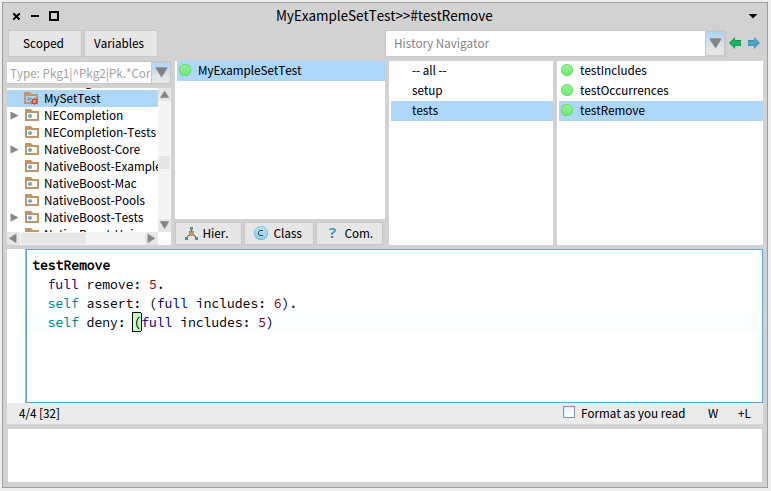
\includegraphics[width=0.8\textwidth]{/Users/ducasse/Workspace/FirstCircle/MyBooks/Bk-Writing/PharoBooks/LearningOOPWithPharoTrans/_result/pdf/Chapters/Tests/figures/updatedbrowsertests.png}\caption{Running SUnit tests from the System Browser: Just click on the round little button close to the class or method.\label{fig:browsertests}}\end{center}
\end{figure}

\subsection{Step 4: Write more tests}
Let's create more tests by defining some methods in the class
\textcode{MyExampleSetTest}.

The second test, named \textcode{testOccurrences}, verifies that the
number of occurrences of 5 in \textcode{full} set is equal to one, even if we
add another element 5 to the set.

\begin{displaycode}{plain}
MyExampleSetTest >> testOccurrences
	| empty full |
	empty := Set new.
	full := Set with: 5 with: 6.
	self assert: (empty occurrencesOf: 0) equals: 0.
	self assert: (full occurrencesOf: 5) equals: 1.
	full add: 5.
	self assert: (full occurrencesOf: 5) equals: 1
\end{displaycode}

Finally, we test that the set no longer contains the element 5 after we have
removed it.

\begin{displaycode}{plain}
MyExampleSetTest >> testRemove
	| full |
	full := Set with: 5 with: 6.
	full remove: 5.
	self assert: (full includes: 6).
	self deny: (full includes: 5)
\end{displaycode}

Note the use of the method \textcode{TestCase \textgreater{}\textgreater{} deny:} to assert something that should
not be true. \textcode{aTest deny: anExpression} is equivalent to
\textcode{aTest assert: anExpression not}, but is much more readable.
\subsection{Step 5: Run all the tests}
You can also select sets of test suites to run, and obtain a more detailed log
of the results using the SUnit Test Runner, which you can open by selecting the menu
\textcode{World \textgreater{} Test Runner}.

The \textit{Test Runner}, shown in Figure \ref{fig:test-runner}, is designed to make it easy to
execute groups of tests.

The left-most pane lists all of the packages that contain test classes (i.e.,
subclasses of \textcode{TestCase}). When some of these packages are selected, the test
classes that they contain appear in the pane to the right. Abstract classes are
italicized, and the test class hierarchy is shown by indentation, so subclasses
of \textcode{ClassTestCase} are indented more than subclasses of \textcode{TestCase}.
\textcode{ClassTestCase} is a class offering utilities methods to compute test
coverage.


\begin{figure}

\begin{center}
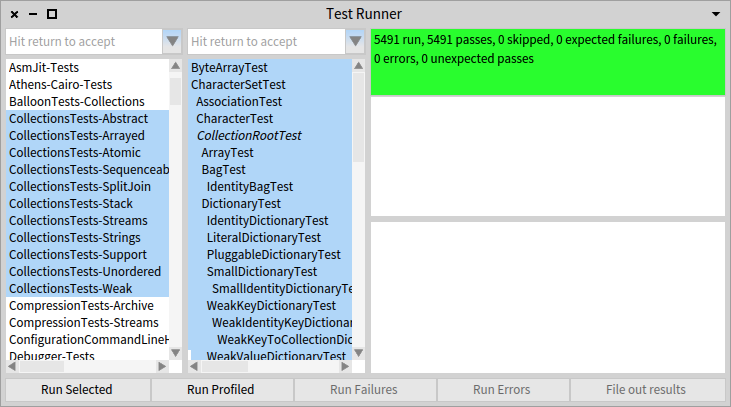
\includegraphics[width=0.8\textwidth]{/Users/ducasse/Workspace/FirstCircle/MyBooks/Bk-Writing/PharoBooks/LearningOOPWithPharoTrans/_result/pdf/Chapters/Tests/figures/updatedtestRunner.png}\caption{Running SUnit tests using the \textit{TestRunner}.\label{fig:test-runner}}\end{center}
\end{figure}


Open a Test Runner, select the package \textit{MySetTest}, and click the \textcode{Run Selected}
button.
\subsection{Step 6: Alternative ways to execute tests}
You can also run a single test (and print the usual pass/fail result summary) by executing a
\textit{Print it} on the following code: \textcode{MyExampleSetTest run: \#testRemove}.

Some people include an executable comment in their test methods as in \textcode{testRemove} below. For example the contents of the comment \textcode{self run: \#testRemove} can be executed: select the expression inside the comment (but not the comment) and bring the menu to do a \textit{Do it}.
It will execute the test. 

\begin{displaycode}{plain}
MyExampleSetTest >> testRemove
	"self run: #testRemove"
	| empty full |
	empty := Set new.
	full := Set with: 5 with: 6.
	full remove: 5.
	self assert: (full includes: 6).
	self deny: (full includes: 5)
\end{displaycode}
\subsection{Step 7: Looking at a bug}
Introduce a bug in \textcode{MyExampleSetTest \textgreater{}\textgreater{} testRemove} and run the tests again. For
example, change \textcode{6} to \textcode{7}, as in:

\begin{displaycode}{plain}
MyExampleSetTest >> testRemove
	| empty full |
	empty := Set new.
	full := Set with: 5 with: 6.
	full remove: 5.
	self assert: (full includes: 7).
	self deny: (full includes: 5)
\end{displaycode}

The tests that did not pass (if any) are listed in the right-hand panes of the
\textit{Test Runner}. If you want to debug one, to see why it failed, just click on
the name. Alternatively, you can execute one of the following expressions:

\begin{displaycode}{plain}
(MyExampleSetTest selector: #testRemove) debug

MyExampleSetTest debug: #testRemove
\end{displaycode}
\subsection{Step 8: Interpret the results}
The method \textcode{assert:} is defined in the class \textcode{TestAsserter}. This is a superclass
of \textcode{TestCase} and therefore all other \textcode{TestCase} subclasses and is responsible for
all kinds of test result assertions.
The \textcode{assert:} method expects a boolean argument, usually the value of a tested expression. When the
argument is true, the test passes; when the argument is false, the test fails.

There are actually three possible outcomes of a test: \textit{passing}, \textit{failing}, and \textit{raising an error}.

\begin{itemize}
\item \textbf{Passing}. The outcome that we hope for is that all of the assertions in the test are true, in which case the test passes. In the test runner, when all of the tests pass, the bar at the top turns green. 
\item \textbf{Failing}. The obvious way is that one of the assertions can be false, causing the test to \textit{fail}.
\item \textbf{Error}. The other possibility is that some kind of error occurs during the execution of the test, such as a \textit{message not understood} error or an \textit{index out of bounds} error. If an error occurs, the assertions in the test method may not have been executed at all, so we can't say that the test has failed; nevertheless, something is clearly wrong!
\end{itemize}

In the \textit{test runner}, failing tests cause the bar at the top to turn yellow, and are listed in the middle pane on
the right, whereas tests with errors cause the bar to turn red, and are listed in
the bottom pane on the right.

As an exercise, modify your tests to provoke both errors and failures.
\section{The SUnit cookbook}
This section will give you more details on how to use SUnit. If you have used
another testing framework such as JUnit, much of this will be familiar, since
all these frameworks have their roots in SUnit. Normally you will use SUnit's
GUI to run tests, but there are situations where you may not want to use it.
\subsection{About assert:equals:}
Note that we either used both \textcode{assert: aBoolean} and \textcode{assert: expression equals: aValue}. The second one provides nicer 
feedback when the assertion fails. The two following lines are equals. 

\begin{displaycode}{plain}
self assert: (empty occurrencesOf: 0) equals: 0.
self assert: (empty occurrencesOf: 0) = 0.
\end{displaycode}

Using \textcode{assert:equals:} provides a better feedback when the test is failing because we
said explicitly that the result should be 0. 
\subsection{Other assertions}
In addition to \textcode{assert:} and \textcode{deny:}, there are several other methods that
can be used to make assertions.

First, \textcode{assert:description:} and \textcode{deny:description:}
take a second argument which is a message string that describes
the reason for the failure, if it is not obvious from the test itself. 

Next, SUnit provides two additional methods, \textcode{should:raise:} and
\textcode{shouldnt:raise:} for testing exception propagation.

For example, you would use \textcode{self should: aBlock raise: anException} to test
that a particular exception is raised during the execution of \textcode{aBlock}. The
method below illustrates the use of \textcode{should:raise:}.

\begin{displaycode}{plain}
MyExampleSetTest >> testIllegal
	| empty |
	self should: [ empty at: 5 ] raise: Error.
	self should: [ empty at: 5 put: #zork ] raise: Error
\end{displaycode}

Try running this test. Note that the first argument of the \textcode{should:} and
\textcode{shouldnt:} methods is a block that contains the expression to be executed.
\subsection{Running a single test}
Normally, you will run your tests using the Test Runner or using your code
browser. If you don't want to launch the Test Runner from the World menu, you
can execute \textcode{TestRunner open}. You can also run a single test as follows:

\begin{displaycode}{plain}
MyExampleSetTest run: #testRemove
>>> 1 run, 1 passed, 0 failed, 0 errors
\end{displaycode}
\subsection{Running all the tests in a test class}
Any subclass of \textcode{TestCase} responds to the message \textcode{suite} and builds
a test suite that contains all the methods whose names start with
the string \textit{test}.

To run the tests in the suite, send it the message \textcode{run}. For example:

\begin{displaycode}{plain}
MyExampleSetTest suite run 
>>> 5 run, 5 passed, 0 failed, 0 errors
\end{displaycode}
\subsection{Must I subclass TestCase?}
In JUnit you can build a TestSuite from an arbitrary class containing \textcode{test*}
methods. In SUnit you can do the same but you will then have to create a suite
by hand and your class will have to implement all the essential \textcode{TestCase}
methods like \textcode{assert:}. We recommend, however, that you not try to do this.
The framework is there: use it.
\section{Defining a fixture}
In the previous example, we defined the context in each test methods and it was a bit boring to 
duplicate all the logic in any tests. In fact SUnit proposes a solution to this.
\subsection{Step 1: Define the class and context}
We can define the context using the two instance variables \textcode{full} and \textcode{empty} that
we will use to represent a full and an empty set. 

\begin{displaycode}{plain}
TestCase subclass: #MyExampleSetTest
	instanceVariableNames: 'full empty'
	classVariableNames: ''
	package: 'MySetTest'
\end{displaycode}
\subsection{Step 2: Setting a reusable context}
The method \textcode{TestCase \textgreater{}\textgreater{} setUp} defines the context in which each of  the tests will run.
 The message \textcode{setUp} is sent before the execution of each test method defined in the test class.

Define the \textcode{setUp} method as follows, to initialize the \textcode{empty} variable to
refer to an empty set and the \textcode{full} variable to refer to a set containing two
elements. 

\begin{displaycode}{plain}
MyExampleSetTest >> setUp
	empty := Set new.
	full := Set with: 5 with: 6
\end{displaycode}

In testing jargon the context is called the \textit{fixture} for the test.
\subsection{Step 3: Write some test methods}
Now the previous tests methods are much more compact and contain less duplication.

\begin{displaycode}{plain}
MyExampleSetTest >> testIncludes
	self assert: (full includes: 5).
	self assert: (full includes: 6)
\end{displaycode}

\begin{displaycode}{plain}
MyExampleSetTest >> testOccurrences
	self assert: (empty occurrencesOf: 0) equals: 0.
	self assert: (full occurrencesOf: 5) equals: 1.
	full add: 5.
	self assert: (full occurrencesOf: 5) equals: 1
\end{displaycode}

\begin{displaycode}{plain}
MyExampleSetTest >> testRemove
	full remove: 5.
	self assert: (full includes: 6).
	self deny: (full includes: 5)
\end{displaycode}
\section{Chapter summary}
This chapter explained why tests are an important investment in the future of
your code. We explained in a step-by-step fashion how to define a few tests for
the class \textcode{Set}. 

\begin{itemize}
\item To maximize their potential, unit tests should be fast, repeatable, independent of any direct human interaction and cover a single unit of functionality.
\item Tests for a class called \textcode{MyClass} belong in a class named \textcode{MyClassTest}, which should be introduced as a subclass of \textcode{TestCase}.
\item Initialize your test data in a \textcode{setUp} method.
\item Each test method should start with the word \textit{test}.
\item Use the \textcode{TestCase} methods \textcode{assert:}, \textcode{deny:} and others to make assertions.
\item Run tests!
\end{itemize}

As exercise, turn the examples given in the first chapter into tests.



% lulu requires an empty page at the end. That's why I'm using
% \backmatter here.
\backmatter

% Index would go here
\bibliographystyle{abbrv}
\bibliography{others.bib}
\end{document}
